\documentclass{../praktikum-protokollvorlage-latex/include/protokollclassE}
\SelectLanguage{english}

\newcommand{\praktikum}{P2}
\newcommand{\semester}{SS17}

\newcommand{\wochentag}{Do}
\newcommand{\gruppennr}{07}

\newcommand{\nachnamea}{Elicabuk}
\newcommand{\vornamea}{Umut}
\newcommand{\nachnameb}{Pittermann}
\newcommand{\vornameb}{Martin}

\input{../common/emails.tex}

\hyphenation
{
	über-nom-me-nen
	an-ge-ge-be-nen
}

\newcommand{\maketitlepage}
{
	% coordinates for background border
\newcommand{\diameter}{20}
\newcommand{\xone}{-15}
\newcommand{\xtwo}{160}
\newcommand{\yone}{15}
\newcommand{\ytwo}{-253}

\newcommand{\hoehea}{60}
\newcommand{\hoeheb}{60}




\begin{titlepage}
    % background border
    \begin{tikzpicture}[overlay]
    \draw[color=gray]  
            (\xone mm, \yone mm)
      -- (\xtwo mm, \yone mm)
    arc (90:0:\diameter pt) 
      -- (\xtwo mm + \diameter pt , \ytwo mm) 
        -- (\xone mm + \diameter pt , \ytwo mm)
    arc (270:180:\diameter pt)
        -- (\xone mm, \yone mm);
    \end{tikzpicture}
    
    % KIT logo
    \begin{textblock}{10}[0,0](4.5,2.5)
        
\includegraphics[width=.25\textwidth]{../praktikum-protokollvorlage-latex/include/kitlogo.pdf}
    \end{textblock}
    \changefont{phv}{m}{n}    % helvetica
    \begin{textblock}{10}[0,0](5.5,2.2)
        \begin{flushright}
            \Large FAKULTÄT FÜR PHYSIK\\Praktikum Klassische Physik
        \end{flushright}
    \end{textblock}
    
    \begin{textblock}{10}[0,0](4.2,3.1)
        \begin{tikzpicture}[overlay]
        \draw[color=gray]
            (\xone mm + 5 mm, -12 mm)
         -- (\xtwo mm + \diameter pt - 5 mm, -12 mm);
        \end{tikzpicture}
    \end{textblock}
    
    \Large
    % Zeile 1
    \begin{textblock}{12}[0,0](3.58,4.4)
        \mytextfield{Prak.}{\praktikum}{0.9cm}{17pt}
                    {P1/P2}{2}{Praktikum}
    \end{textblock}
    \begin{textblock}{12}[0,0](5.53,4.4)
        \mytextfield{Semester}{\semester}{2.6cm}{17pt}
        {z.B. \glqq WS14/15\grqq\ oder \glqq SS15\grqq}{0}{Semester}
    \end{textblock}
    \begin{textblock}{12}[0,0](9.53,4.4)
        \mytextfield{Wochentag}{\wochentag}{1.3cm}{17pt}
                    {Mo/Di/Mi/Do}{2}{Wochentag}
    \end{textblock}
    \begin{textblock}{12}[0,0](12.88,4.4)
       \mytextfield{Gruppennr.}{\gruppennr}{1.06cm}{17pt}
                   {\#\#}{2}{Gruppennummer}
    \end{textblock}
    
    % Zeile 2
    \begin{textblock}{12}[0,0](3.58,4.95)
        \mytextfield{Name}{\nachnamea}{6cm}{17pt}
                    {}{0}{Name1}
    \end{textblock}
    \begin{textblock}{12}[0,0](9.53,4.95)
        \mytextfield{Vorname}{\vornamea}{6cm}{17pt}
                    {}{0}{Vorname1}
    \end{textblock}
    
    % Zeile 3
    \begin{textblock}{12}[0,0](3.58,5.5)
        \mytextfield{Name}{\nachnameb}{6cm}{17pt}
                    {}{0}{Name2}
    \end{textblock}
    \begin{textblock}{12}[0,0](9.53,5.5)
        \mytextfield{Vorname}{\vornameb}{6cm}{17pt}
                    {}{0}{Vorname2}
    \end{textblock}
    
    % Zeile 4
    \begin{textblock}{12}[0,0](3.64,6.05)
       \normalsize\mytextfield{Emailadresse(n)}{\emailadressen}{13.1cm}{10pt}
                              {Optional}{0}{Emailadressen}
    \end{textblock}
    
    % Zeile 5
    \begin{textblock}{12}[0,0](3.58,7)
        \mytextfield{Versuch}{\versuch\ (\praktikum-\versuchsnr)}{9.45cm}{14pt}
                    {z.B. \glqq Galvanometer (P1-13)\grqq\ oder \glqq %
                     Mikrowellenoptik (P2-15)\grqq}{0}{Versuch}
    \end{textblock}
    \begin{textblock}{12}[0,0](12.58,7)
       \mytextfield{Fehlerrech.}{\fehlerrechnung}{1.46cm}{17pt}
                   {Ja/Nein}{4}{Fehlerrechnung}
    \end{textblock}
    
    % Zeile 6
    \begin{textblock}{12}[0,0](3.58,7.55)
        \mytextfield{Betreuer}{\betreuer}{7cm}{17pt}{}{0}{Betreuer}
    \end{textblock}
    \begin{textblock}{12}[0,0](10.82,7.55)
        \mytextfield{Durchgeführt am}{\durchgefuehrt}{2.53cm}{17pt}
                    {TT.MM.JJ}{8}{Durchfuehrung}
    \end{textblock}
    
    % Querstrich
    \begin{textblock}{20}[0,0](0,7.9)\tiny\centering
        Wird vom Betreuer ausgefüllt.
    \end{textblock}
    \begin{tikzpicture}[overlay]
    \draw[color=gray]
        (\xone mm + 5 mm, -95 mm)
     -- (\xtwo mm + \diameter pt - 5 mm, -95 mm);
    \end{tikzpicture}
    
    % Zeile 1
    \begin{textblock}{12}[0,0](3.65,8.57)
        \myTtextfield{1. Abgabe am}{}{2.5cm}{17pt}
                     {}
    \end{textblock}
    
    % Block 1
    \begin{tikzpicture}[overlay]
    \draw[color=gray]  
        (\xone mm + 10 mm, -107.5 mm)
     -- (\xtwo mm + \diameter pt - 10 mm, -107.5 mm)
     -- (\xtwo mm + \diameter pt - 10 mm, -107.5 mm - \hoehea mm)
     -- (\xone mm + 10 mm, -107.5 mm - \hoehea mm)
     -- (\xone mm + 10 mm, -107.5 mm);
    \end{tikzpicture}
    \begin{textblock}{20}[0,0](3.8,9.2)
        \myTtextfield{Rückgabe am}{}{2.5cm}{17pt}
                     {}
    \end{textblock}
    \begin{textblock}{20}[0,0](8.7,9.2)
        \smash{Begründung:}
    \end{textblock}
    
    % Zeile 2
    \begin{textblock}{12}[0,0](3.65,12.6)
        \myTtextfield{2. Abgabe am}{}{2.5cm}{17pt}
                     {}
    \end{textblock}
    
    % Block 2
    \begin{tikzpicture}[overlay]
    \draw[color=gray]  
        (\xone mm + 10 mm, -180 mm)
     -- (\xtwo mm + \diameter pt - 10 mm, -180 mm)
     -- (\xtwo mm + \diameter pt - 10 mm, -180 mm - \hoehea mm)
     -- (\xone mm + 10 mm, -180 mm - \hoehea mm)
     -- (\xone mm + 10 mm, -180 mm);
    \end{tikzpicture}
    \begin{textblock}{12}[0,0](4,13.25)
        \smash{Ergebnis:~~~~+~~~/~~~0~~~/~~~-}
    \end{textblock}
    \begin{textblock}{12}[0,0](9.5,13.25)
        \smash{Fehlerrechnung:~~~Ja~~~/~~~Nein}
    \end{textblock}
    \begin{textblock}{12}[0,0](3.8,13.72)
        \myTtextfield{Datum}{}{2.5cm}{17pt}
                     {}
    \end{textblock}
    \begin{textblock}{12}[0,0](8.3,13.72)
        \myTtextfield{Handzeichen}{}{5.5cm}{17pt}
                     {}
    \end{textblock}
    \begin{textblock}{12}[0,0](4,14.25)\Large
        \smash{Bemerkungen:}
    \end{textblock}
    
    
    
    % lowest text blocks concerning the KIT
    \begin{textblock}{10}[0,0](4,16.8)
        \tiny{KIT -- Universität des Landes Baden-Württemberg und nationales %
              Forschungszentrum in der Helmholtz-Gemeinschaft}
    \end{textblock}
    \begin{textblock}{10}[0,0](14,16.75)
        \large{\textbf{www.kit.edu}}
    \end{textblock}
\end{titlepage}

	\begingroup \let\clearpage\relax
	\tableofcontents
	\listoffigures
	\listoftables
	\endgroup
}

\newcommand{\configureappendix}
{
	\chapter*{\appendixname} \addcontentsline{toc}{chapter}{\appendixname}
}

\newcommand{\s}[1]{\ensuremath{_\text{#1}}}


\newcommand{\versuch}{Ideal And Real Gases}
\newcommand{\versuchsnr}{47}			%P!- weglassen
\newcommand{\fehlerrechnung}{Ja}

\newcommand{\betreuer}{Janek Bechtel}
\newcommand{\durchgefuehrt}{22.06.17}
\newcommand{\at}[2][]{#1|_{#2}}

\usepackage{xfrac}
\begin{document}
	\FrontMatter
	% coordinates for background border
\newcommand{\diameter}{20}
\newcommand{\xone}{-15}
\newcommand{\xtwo}{160}
\newcommand{\yone}{15}
\newcommand{\ytwo}{-253}

\newcommand{\hoehea}{60}
\newcommand{\hoeheb}{60}




\begin{titlepage}
    % background border
    \begin{tikzpicture}[overlay]
    \draw[color=gray]  
            (\xone mm, \yone mm)
      -- (\xtwo mm, \yone mm)
    arc (90:0:\diameter pt) 
      -- (\xtwo mm + \diameter pt , \ytwo mm) 
        -- (\xone mm + \diameter pt , \ytwo mm)
    arc (270:180:\diameter pt)
        -- (\xone mm, \yone mm);
    \end{tikzpicture}
    
    % KIT logo
    \begin{textblock}{10}[0,0](4.5,2.5)
        
\includegraphics[width=.25\textwidth]{../praktikum-protokollvorlage-latex/include/kitlogo.pdf}
    \end{textblock}
    \changefont{phv}{m}{n}    % helvetica
    \begin{textblock}{10}[0,0](5.5,2.2)
        \begin{flushright}
            \Large FAKULTÄT FÜR PHYSIK\\Praktikum Klassische Physik
        \end{flushright}
    \end{textblock}
    
    \begin{textblock}{10}[0,0](4.2,3.1)
        \begin{tikzpicture}[overlay]
        \draw[color=gray]
            (\xone mm + 5 mm, -12 mm)
         -- (\xtwo mm + \diameter pt - 5 mm, -12 mm);
        \end{tikzpicture}
    \end{textblock}
    
    \Large
    % Zeile 1
    \begin{textblock}{12}[0,0](3.58,4.4)
        \mytextfield{Prak.}{\praktikum}{0.9cm}{17pt}
                    {P1/P2}{2}{Praktikum}
    \end{textblock}
    \begin{textblock}{12}[0,0](5.53,4.4)
        \mytextfield{Semester}{\semester}{2.6cm}{17pt}
        {z.B. \glqq WS14/15\grqq\ oder \glqq SS15\grqq}{0}{Semester}
    \end{textblock}
    \begin{textblock}{12}[0,0](9.53,4.4)
        \mytextfield{Wochentag}{\wochentag}{1.3cm}{17pt}
                    {Mo/Di/Mi/Do}{2}{Wochentag}
    \end{textblock}
    \begin{textblock}{12}[0,0](12.88,4.4)
       \mytextfield{Gruppennr.}{\gruppennr}{1.06cm}{17pt}
                   {\#\#}{2}{Gruppennummer}
    \end{textblock}
    
    % Zeile 2
    \begin{textblock}{12}[0,0](3.58,4.95)
        \mytextfield{Name}{\nachnamea}{6cm}{17pt}
                    {}{0}{Name1}
    \end{textblock}
    \begin{textblock}{12}[0,0](9.53,4.95)
        \mytextfield{Vorname}{\vornamea}{6cm}{17pt}
                    {}{0}{Vorname1}
    \end{textblock}
    
    % Zeile 3
    \begin{textblock}{12}[0,0](3.58,5.5)
        \mytextfield{Name}{\nachnameb}{6cm}{17pt}
                    {}{0}{Name2}
    \end{textblock}
    \begin{textblock}{12}[0,0](9.53,5.5)
        \mytextfield{Vorname}{\vornameb}{6cm}{17pt}
                    {}{0}{Vorname2}
    \end{textblock}
    
    % Zeile 4
    \begin{textblock}{12}[0,0](3.64,6.05)
       \normalsize\mytextfield{Emailadresse(n)}{\emailadressen}{13.1cm}{10pt}
                              {Optional}{0}{Emailadressen}
    \end{textblock}
    
    % Zeile 5
    \begin{textblock}{12}[0,0](3.58,7)
        \mytextfield{Versuch}{\versuch\ (\praktikum-\versuchsnr)}{9.45cm}{14pt}
                    {z.B. \glqq Galvanometer (P1-13)\grqq\ oder \glqq %
                     Mikrowellenoptik (P2-15)\grqq}{0}{Versuch}
    \end{textblock}
    \begin{textblock}{12}[0,0](12.58,7)
       \mytextfield{Fehlerrech.}{\fehlerrechnung}{1.46cm}{17pt}
                   {Ja/Nein}{4}{Fehlerrechnung}
    \end{textblock}
    
    % Zeile 6
    \begin{textblock}{12}[0,0](3.58,7.55)
        \mytextfield{Betreuer}{\betreuer}{7cm}{17pt}{}{0}{Betreuer}
    \end{textblock}
    \begin{textblock}{12}[0,0](10.82,7.55)
        \mytextfield{Durchgeführt am}{\durchgefuehrt}{2.53cm}{17pt}
                    {TT.MM.JJ}{8}{Durchfuehrung}
    \end{textblock}
    
    % Querstrich
    \begin{textblock}{20}[0,0](0,7.9)\tiny\centering
        Wird vom Betreuer ausgefüllt.
    \end{textblock}
    \begin{tikzpicture}[overlay]
    \draw[color=gray]
        (\xone mm + 5 mm, -95 mm)
     -- (\xtwo mm + \diameter pt - 5 mm, -95 mm);
    \end{tikzpicture}
    
    % Zeile 1
    \begin{textblock}{12}[0,0](3.65,8.57)
        \myTtextfield{1. Abgabe am}{}{2.5cm}{17pt}
                     {}
    \end{textblock}
    
    % Block 1
    \begin{tikzpicture}[overlay]
    \draw[color=gray]  
        (\xone mm + 10 mm, -107.5 mm)
     -- (\xtwo mm + \diameter pt - 10 mm, -107.5 mm)
     -- (\xtwo mm + \diameter pt - 10 mm, -107.5 mm - \hoehea mm)
     -- (\xone mm + 10 mm, -107.5 mm - \hoehea mm)
     -- (\xone mm + 10 mm, -107.5 mm);
    \end{tikzpicture}
    \begin{textblock}{20}[0,0](3.8,9.2)
        \myTtextfield{Rückgabe am}{}{2.5cm}{17pt}
                     {}
    \end{textblock}
    \begin{textblock}{20}[0,0](8.7,9.2)
        \smash{Begründung:}
    \end{textblock}
    
    % Zeile 2
    \begin{textblock}{12}[0,0](3.65,12.6)
        \myTtextfield{2. Abgabe am}{}{2.5cm}{17pt}
                     {}
    \end{textblock}
    
    % Block 2
    \begin{tikzpicture}[overlay]
    \draw[color=gray]  
        (\xone mm + 10 mm, -180 mm)
     -- (\xtwo mm + \diameter pt - 10 mm, -180 mm)
     -- (\xtwo mm + \diameter pt - 10 mm, -180 mm - \hoehea mm)
     -- (\xone mm + 10 mm, -180 mm - \hoehea mm)
     -- (\xone mm + 10 mm, -180 mm);
    \end{tikzpicture}
    \begin{textblock}{12}[0,0](4,13.25)
        \smash{Ergebnis:~~~~+~~~/~~~0~~~/~~~-}
    \end{textblock}
    \begin{textblock}{12}[0,0](9.5,13.25)
        \smash{Fehlerrechnung:~~~Ja~~~/~~~Nein}
    \end{textblock}
    \begin{textblock}{12}[0,0](3.8,13.72)
        \myTtextfield{Datum}{}{2.5cm}{17pt}
                     {}
    \end{textblock}
    \begin{textblock}{12}[0,0](8.3,13.72)
        \myTtextfield{Handzeichen}{}{5.5cm}{17pt}
                     {}
    \end{textblock}
    \begin{textblock}{12}[0,0](4,14.25)\Large
        \smash{Bemerkungen:}
    \end{textblock}
    
    
    
    % lowest text blocks concerning the KIT
    \begin{textblock}{10}[0,0](4,16.8)
        \tiny{KIT -- Universität des Landes Baden-Württemberg und nationales %
              Forschungszentrum in der Helmholtz-Gemeinschaft}
    \end{textblock}
    \begin{textblock}{10}[0,0](14,16.75)
        \large{\textbf{www.kit.edu}}
    \end{textblock}
\end{titlepage}

	\maketitlepage

	\MainMatter


	\chapter{Absolute Zero}

The temperature of absolute zero is determined by measuring thermal expansion of a gas and extrapolating to the point of zero pressure.

According to the ideal gas law
\begin{equation}\label{eq:ideal-gas}
	pV = nRT,
\end{equation}
pressure $p$ is proportional to (absolute) temperature $T$.
To relate absolute temperature to the celsius scale, which differs by a constant temperature offset $T_\text{o}$: $T_\text{C} \, (\si{\celsius}) = T \, (\si{\kelvin}) - T_\text{o}$, a modified version of \autoref{eq:ideal-gas},
\begin{equation*}
	p(T) = p_0 \cdot \left(1 + \alpha \, T_\text{C}\right),
\end{equation*}
is used.
The point of zero pressure in the units of $T_\text{c}$ is $T_\text{o} = -\frac{1}{\alpha}$.

As $p(T)$ is purely linear, two points $(p, T)$ are sufficient to calculate $\alpha$.
In the experiment two easily reproducible temperatures, the melting and boiling point of water, are used.

To correct for the temperature dependent boiling point of water, the ambient pressure is measured:
\begin{equation*}
	p_\text{A} = \SI{996}{\milli\bar} \quad \rightarrow \quad T_\mathrm{b, H_2O} = \SI{99.49}{\celsius}\footnote{\url{http://www.wolframalpha.com/input/?i=water+boiling+point+996mBar}}.
\end{equation*}

To calculate the error on $\alpha$, uncertainties of $\Delta p = \SI{1}{\mmHg}$ on the relative pressure, $\Delta T_\text{b} = \SI{2}{\celsius}$ on the boiling temperature (and $\Delta p_\text{A} = \SI{5}{\milli\bar}$ on the ambient pressure) are assumed.
All error sources are uncorrelated, so gaussian error propagation is used.

$\alpha_1$ is calculated from the two data points as
\begin{equation*}
	\alpha_1 = \frac{p_\text{b} - p_0}{p_0 \cdot T_\text{b}} = \SI{3.716(78)e-3}{\per\celsius},
\end{equation*}
with the pressure $p_0$ at \SI{0}{\celsius} and the pressure $p_\text{b}$ and temperature $T_\text{b}$ (in \si{\celsius}) at the boiling point of water.

The effects of thermal expansion of the test vessel are corrected:
\begin{equation*}	%http://www.wolframalpha.com/input/?i=264mmHg%2F(996mBar*99.45%C2%B0C)+%2B+2.5e-5%2Fcelsius+*+(231mmHg+%2B+996mBar)%2F996mBar
	\alpha = \alpha_1 + \frac{p_\text{b}}{p_0} \cdot \gamma = \SI{3.750(78)e-3}{\per\celsius},
\end{equation*}
which corresponds to a zero point of \SI{-266.6(56)}{\celsius}.

The actual value (by definition) of $T_\text{o} = \SI{-273.15}{\celsius}$ does not lie within the calculated error bounds.
An additional error source is the air volume outside of the water bath which acts as a buffer for pressure changes, which can't be accounted for without analyzing the thermal conductivity of the apparatus.

\begin{table}
	\centering
	\caption{\textbf{relative air pressure} in test vessel with fixed volume at various temperatures, pressure relative to $p_\text{A} = \SI{996}{\milli\bar}$}
	\begin{tabular}{cS}
		\toprule
		condition&
		{relative pressure (\si{\mmHg})}\\
		\midrule
		ambient (\SI{27.6}{\celsius})&	42\\
		freezing&	-33\\
		boiling&	231\\
		\bottomrule
	\end{tabular}
\end{table}

	\chapter{Heat Capacity Ratio $\kappa$}

Adiabatic processes in ideal gases can be described with the polytropic process equations
\begin{equation}
	pV^\kappa = \text{const} \quad \text{and} \quad TV^{\kappa - 1} = \text{const},
\end{equation}
where $\kappa = \frac{c_\text{p}}{c_\text{v}}$ is the ratio of the specific heat capacities for constant pressure and volume.

\begin{figure}[tbp]
	\centering
	\includegraphics[width=.8\textwidth]{data/plots/2_img.pdf}
	\caption[Clément-Desormes $p(V)$ Diagram]{$p(V)$ diagram of working gas for determining $\kappa$ (after Clément-Desormes)}
	\label{fig:pv-clement-method}
\end{figure}

In this experiment $\kappa$ is determined using the method described by Clément-Desormes:
\begin{itemize}
	\item A sealed constainer is pressurized and let cool down to ambient temperature\\
	\mbox{$\rightarrow (p_0 + dp_1, V_0, T_0)$}
	\item The container is opened briefly to let the pressure escape\\
	\mbox{$\rightarrow (p_0, V_0, T_0 - dT)$}
	\item The gas that was cooled down in the expansion process heats up to room temperature again\\
	\mbox{$\rightarrow (p_0 + dp_2, V_0, T_0)$}
\end{itemize}
The $p(V)$ diagram of this process is shown in \autoref{fig:pv-clement-method}.

Assuming $dp_x \ll p_0$, $\kappa$ can be calculated\footnote{Vorbereitungshilfe zum Versuch „Ideales und Reales Gas“} as
\begin{equation}
	\kappa = \frac{dp_1}{dp_1 - dp_2} = \frac{dh_1}{dh_1 - dh_2},
\end{equation}
where $dh_x$ denotes the height difference of the fluid levels in the two arms of the manometer, the density of the used liquid cancels out.

In this very much simplified equation, only the read-off error must be considered.
As the manometer was levelled with a bubble level and the two arms of the u tube are very close together, any systematic offset of pressures is small enough to be disregarded.
For the statistical read-off error on $dh_x$ an error of \SI{2}{\milli\meter} is assumed, the errors on $dh_1$ and $dh_2$ are combined with gaussian error propagation.

The experiment is repeated three times with varying initial pressure $dp_1$.
The values along with individual results for $\kappa$ and associated uncertainties are listed in \autoref{tab:kappa}.

The mean value is $\bar{\kappa} = \num{1.27(2)}$, which deviates from the literature value\footnote{\url{webbook.nist.gov/chemistry/fluid/}} of $\kappa_\text{lit} = \num{1.40}$ ($\text{N}_2$ at \SI{20}{\celsius}) by \SI{10}{\percent}.

This is probably due to the slow venting process, where a lot of pressure that comes from re-heating the gas to ambient temperature is lost.
This is confirmed by a second experiment where the vent is purposefully left open for longer than neccessary.
The resulting pressure $dp_2$ is significantly smaller than in the previous tests.
The low variance between the results implicates a very consistent venting process which, being carried out by hand, was not expected.

\begin{table}
	\centering
	\caption[Clément-Desormes Method Values]{Results of Clément-Desormes method. $dh_1$ before venting, $dh_2$ after venting and temperature equalization}\label{tab:kappa}
	\begin{tabular}{SSS}
		\toprule
		{$dh_1$ (\si{\mm})}&
		{$dh_2$ (\si{\mm})}&
		{$\kappa$}\\
		\midrule
		112.5&	23&	1.26(3)\\
		79.5&	17&	1.27(4)\\
		91.5&	20.5&	1.28(4)\\
		\bottomrule
	\end{tabular}
	\caption*{$\pm\SI{2}{\mm}$ on all heights measurements}
\end{table}

	\chapter{Adiabatic Exponent Of Air}
This experiment is used to determine the adiabatic exponent of air, based on \texttt{Rüchardt}'s method.

\section{Theory}
A relatively heavy glass cylinder is placed on top of a gas volume \todo{held captive by a terroristic glass bottle}.
This cylinder is excited to vibrations.
As the frequency of these vibrations tend to be too high to be measured by eye, a combination of a coil, a magnet and a frequency counter is used as an electronic solution.

The periodic expansion/compression of this gas is approximately adiabatic. It holds
\begin{align}
	&pV^{\kappa} &&= \text{const.}& \nonumber \\
	\Leftrightarrow\ &\d p &&= -\kappa\cdot p\frac{\d V}{V}&&|\cdot A \nonumber \\
	\Leftrightarrow\ &\d F &&= -\kappa A^2\cdot\frac{p}{V}\cdot\d x &&\text{(using $A\cdot \d p=\d F$ and $A\cdot\d x=\d V$).} \label{eq:adiabatic_df}
\end{align}\todo{fix shitty left alignment of align}

\autoref{eq:adiabatic_df} is a linear law with a eigenfrequency of
\begin{align*}
	f&=\frac{1}{2\pi}\sqrt{\frac{k}{m}},
\end{align*}
where $k=\kappa A^2\cdot\sfrac{p}{V}$.
This results in
\begin{align}\label{eq:kappa}
	\kappa&=\left(\frac{2\pi f}{A}\right)^2\cdot\frac{mV}{p},
\end{align}
where\par
\begin{tabular}{ll}
	$f-$	&	frequency of oscillation \\
	$m-$	&	cylinder mass (including magnet) \\
	$A-$	&	cross section \\
	$V-$	&	gas volume \\
	$p-$	&	gas pressure (accounting for magnet mass)\\
\end{tabular}\par
denote the characteristic properties of the experiment.

	\chapter{Vapor Pressure Curve Of N-Hexane}
This exerpiment explores the evaporation enthalpy of n-hexane and its associated vapor pressure curve.

\section{Theory}
\begin{figure}[tbp]
	\centering
	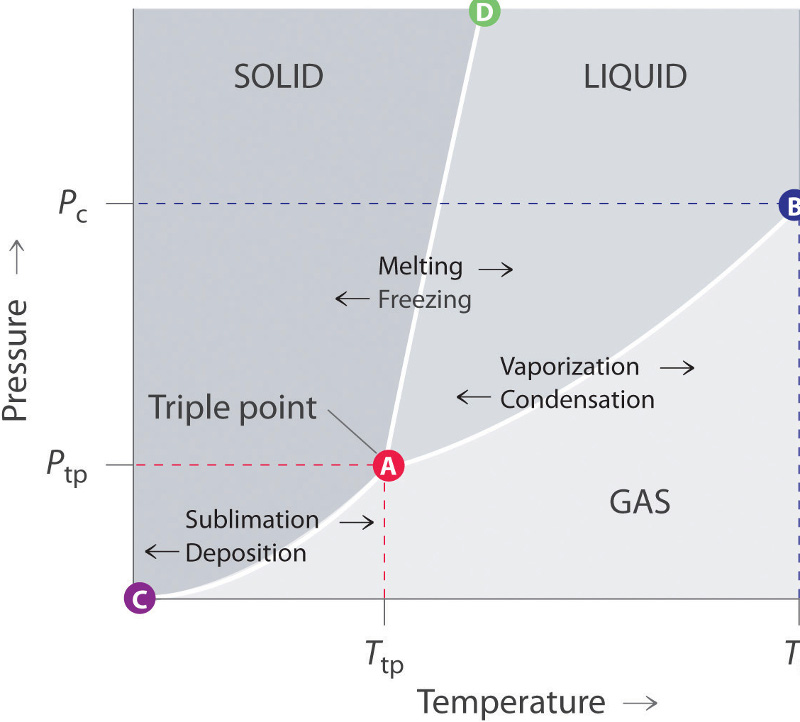
\includegraphics[width=.4\textwidth]{./img/phase.jpg}
	\caption[Phase diagram of n-hexane]{\textbf{Phase diagram of n-hexane} The vapor pressure curve can be seen between the gaseous and liquid phase\newline Source:\url{saylordotorg.github.io/text_general-chemistry-principles-patterns-and-applications-v1.0/s15-07-phase-diagrams.html}}
	\label{fig:n_hexane_phase_diagram}
\end{figure}

A container filled with n-hexane is placed inside of a water bath.
The water bath is heated up and let cool down afterwards.
During both processes, the vapor pressure $p$ and temperature $T$ are measured in regular intervals.

\autoref{fig:n_hexane_phase_diagram} shows the phase diagram of n-hexane.
Unlike water, it is a substance which does not show negative thermal expansion.
The curve between liquid and vapor phase is called the vapor pressure curve.
Points on it are in phase equilibrium, which means that the same amount of vapor condensates as water evaporates.

Using \texttt{Clausius-Clepeyron}'s equation, the evaporation enthalpy $\Lambda$ can be calculated as
\begin{align}\label{eq:evap_enth}
	\Lambda&=T\cdot\left(V_\text{g}-V_\text{l}\right)\cdot\frac{\d p}{\d T} \nonumber \\
	&=TV_\text{g}\cdot\frac{\d p}{\d T}\quad(V_\text{g}\gg V_\text{l})
\end{align}
where $V_\text{g}$ and $V_\text{l}$ denote the gaseous and liquid volume respectively.

Using the ideal gas law, $V_\text{g}$ can be expressed as
\begin{equation}\label{eq:gas_law}
	V_\text{g}\at[\bigg]{n=1}=\frac{RT}{p},
\end{equation}
where $R$ is the universal gas constant $(=\SI{8.31}{\joule\per\mole\kelvin}$).

Combining equations \ref{eq:evap_enth} and \ref{eq:gas_law}, we get the differential equation
\begin{equation}\label{eq:dgl}
	\Lambda=\frac{RT^2}{p}\cdot\frac{\d p}{\d T}.
\end{equation}
Solving \autoref{eq:dgl} yields
\begin{align}
	\frac{\Lambda}{T}&=-R\cdot\log{p}+\text{const.} \nonumber \\
	\Leftrightarrow\ \log{p}&=-\frac{\Lambda}{R}\cdot \frac{1}{T} + \text{const.}	\label{eq:fit_eq} \\
	\Leftrightarrow\ y&=a\cdot x + \text{const.} \nonumber
\end{align}

$\Lambda$ can be determined by fitting this linear model to acquired data $(\frac{1}{T},p)$.

\section{Evaluation}
\begin{figure}[tbp]
	\centering
	\begin{subfigure}{0.4\textwidth}
		\centering
		\includegraphics[width=.9\linewidth]{./data/plots/4_vapor.pdf}
		\caption{\textbf{Measured vapor pressure curve of n-hexane}}
		\label{subfig:press_curve_meas}
	\end{subfigure}
	\begin{subfigure}{0.4\textwidth}
		\centering
		\includegraphics[width=.9\linewidth]{./data/plots/4_enth.pdf}
		\caption{\textbf{Linear regression for determining $\Lambda$}}
		\label{subfig:lambda_meas}
	\end{subfigure}
	\caption{Measured Vapor Pressure of n-Hexane}
\end{figure}

No errors can be estimated as both measurements $T$ and $p$ have negligable uncertainties.
$T$ is measured with a highly precise, electronic thermometer and the differential height of the manometer's filament $\Delta h$, which is proportional to $p$, is measured with a telescope.
\autoref{subfig:press_curve_meas} shows the measured vapor pressure curves.
\autoref{subfig:lambda_meas} shows the linear regression for determining $\Lambda$.
Fitting the model in \autoref{eq:fit_eq} to the data yields the parameters
\begin{align*}
	a_\text{cool}=\SI{-1701(297)}{\kelvin},\ a_\text{heat}=\SI{-1605(274)}{\kelvin},
\end{align*}
with $R^2$-values of
\begin{align*}
	R^2_\text{cool}=\num{0.99},\ R^2_\text{heat}=\num{0.99},
\end{align*}
so the model describes the data in an overly sufficient manner.
These slopes yield enthalpy of vaporization coefficients of
\begin{align*}
	\Lambda_\text{cool}&=\SI{14.14(25)}{\kilo\joule\per\mole},\ \Lambda_\text{heat}=\SI{13.34(23)}{\kilo\joule\per\mole}, \\
	\Rightarrow\ \overline{\Lambda}&=\SI{13.74(12)}{\kilo\joule\per\mole}.
\end{align*}
This value deviates from the literature value\footnote{\url{de.wikipedia.org/wiki/N-Hexan}} of $\Lambda_\text{lit}=\SI{28.85}{\kilo\joule\per\mole}$ by \num{52}\%.
This deviation can be explained by the literature value being specified at the normal pressure boiling point, which was not attained in this experiment.


	%%!TEX root = ../10-Specific-Heat-Capacity.tex
\Appendix
\configureappendix

	%\TheBibliography
\bibliographystyle{babalpha}
\bibliography{../common/lit}

\end{document}
